\section{Architecture and components}
\label{sec:arch}
The following chapter describes the individual components developed during this project as well as the interaction required between the components to fulfil the project goal of actuating the model car base on simulation data.
A diagram with the interactions between the components is visible in \autoref{fig:arch}.

The data from the SpeedDreams simulation is first received by the MQTT server on the \texttt{car-control} topic, as described in \autoref{sec:mqtt-car-control}.
The component running on the PandaBoard is subscribed to this MQTT topic and processes the information, see \autoref{sec:panda}.
The resulting commands are then published on the \texttt{car-servo} MQTT topic, described in \autoref{sec:mqtt-car-servo}.
The component running on the Raspberry Pi in turn is responsible for forwarding the commands according to the rules (\autoref{sec:rpi}) the commands to the Servo Control component (\autoref{sec:servo}).


\begin{figure}[h]
    \centering
    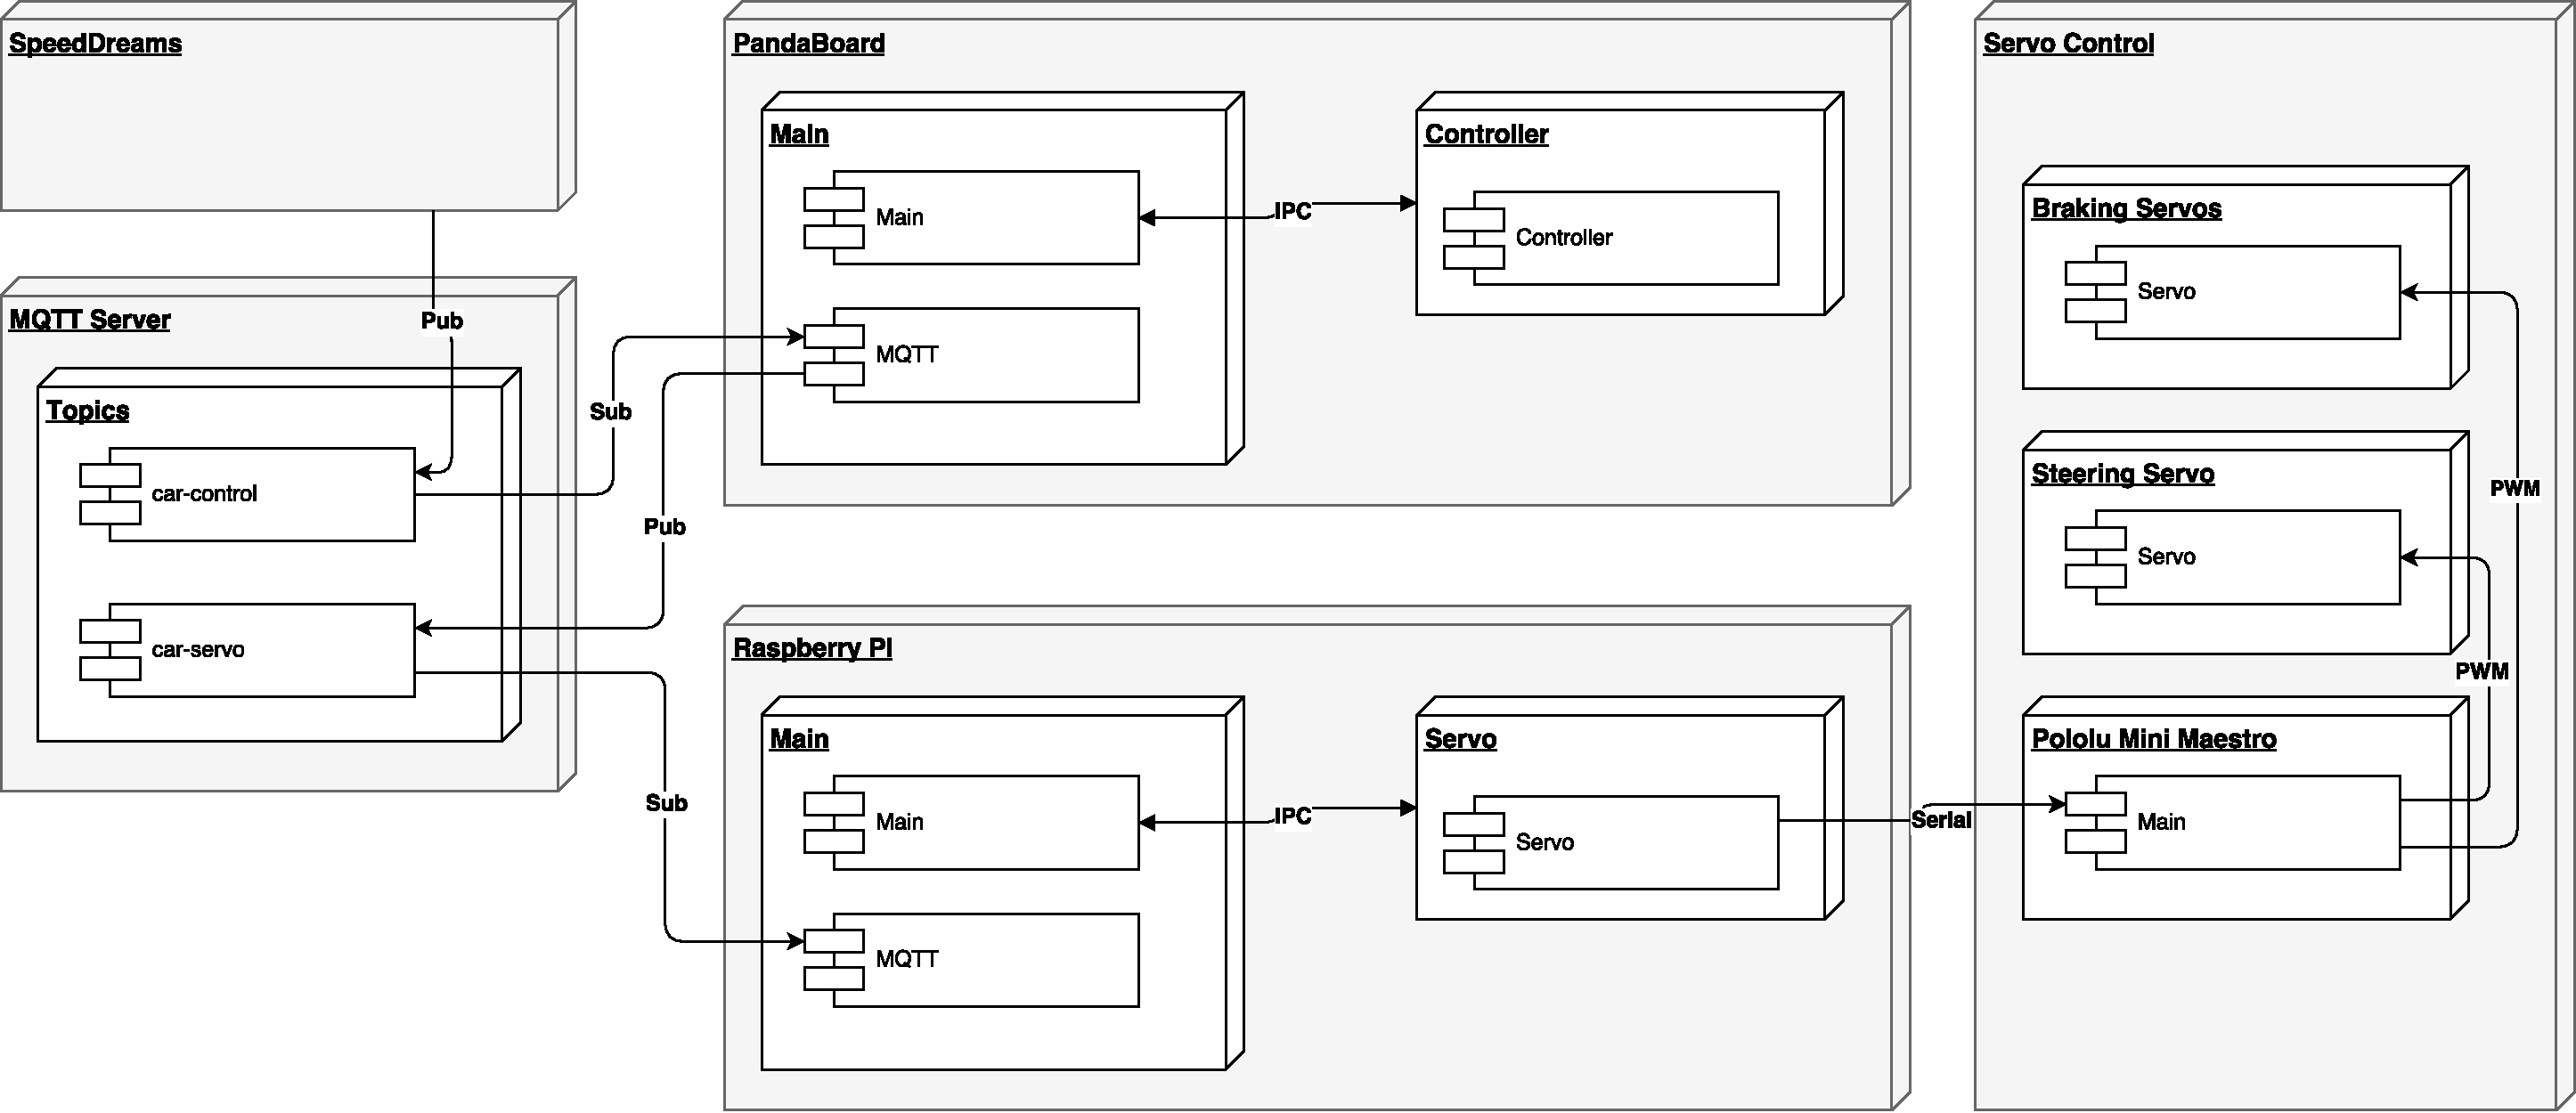
\includegraphics[width=1\linewidth]{images/components}
    \caption{Components overview}
    \label{fig:arch}
\end{figure}

\subsection{Servo (CG)}
\label{sec:servo}
%TODO CG Write chapter

\subsubsection{Requirements}
First of all, all specified requirements except one optional one were fulfilled. In detail the three braking and one steering servos are controlled and the Pololu Maestro Mini Servo Controller Board was connected to them and checked for functionality. The optional requirement to control the main engine was not fulfilled for several reasons. First off all time was running out at the end of the project due to several faced difficulties described in chapter~\ref{sec:challenges}. Furthermore the main engine ca not be controlled by the Pololu Maestro Mini Servo Controller board, because of its power consumption. Instead another more complex controller needs to be used, which requires a serial connection. However Genode as an operating system only supports one serial connection. That is why an additional device would have been needed to be integrated into the setup to control it.

\subsubsection{Hardware Description}
As already described in section~\ref{sec:setup} the used hardware consists of three braking servos, one steering servo and a pololu maestro mini servo controller board, which is displayed in figure~\ref{fig:pololu}.\\

All four servo engines are controlled with a 50Hz pulse width modulation(PWM) signal as is standard for servo engines. The duty cycle of each PWM-signal is between 1 and 2 milliseconds. Because of the nature of the servo controller board, values for the duty cycle of a PWM signal need to be between 4000 and 8000, which corresponds to four times the value in microseconds.\\

\begin{figure}[h!tb]
	\centering
    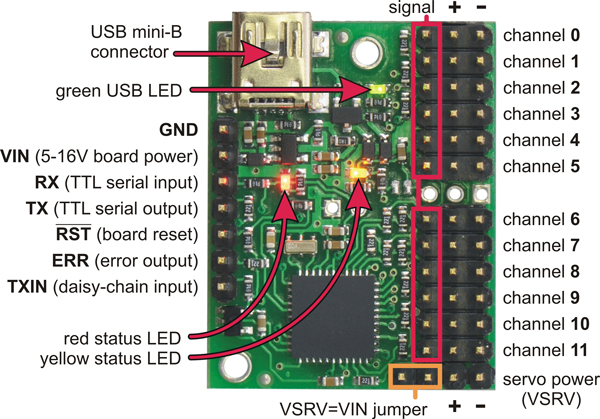
\includegraphics[width=0.7\linewidth]{images/pololu}
    \caption{Pololu Maestro Mini}
    \label{fig:pololu}
\end{figure}

The installed controller board features twelve PWM channels which need to be run on the same frequency but support different duty cycles, so that up to 12 servos could be controlled. For communication with a computer serial communication via USB or UART/TTL on a byte basis can be used. The baudrate for the UART connection is normally autodetected and can be configure. Messages are always sent as eight bits without parity bit and one stop bit(8N1). It also has the capability to execute small script programs. The braking servos are connected to channel 0,1 and 2 and the steering servo is connected to channel 6.\\

Initially the steering servo was not working and therefore was replaced by the chair. Additionally we configured it after its replacement. Also the braking servos were tried to be configured to engage at the same time. However the made improvement was only minor.

\subsubsection{Software Description}
For first testing a shell script and an interactive program with a graphical user interface, both working on all common operating systems, are provided by the supplier and were used. Also some small c example code is provided and was used as a starting point during development. The shell script and the example code is for reference located in the old/pololu folder described in chapter~\ref{sec:scs}.\\

Because of delays in the installation of Genode on the Raspberry Pi that is communicating with the servo controller board, a first program was developed for controlling the servos on Linux, especially Raspbian. The serial port used for communication is exposed as a file in Linux. Therefore commands can be send by writing into the correct file. The program can be found in the old/linux folder as described in chapter~\ref{sec:scs}.\\

All functions provided by the servo class/component have a similar structure. First the input values are checked for valid range, second a command is built and sent and lastly its return value checked for errors. If the servo controller board is supposed to answer, the response is read in, checked for errors and returned. Each command is represented as a char array, where the 7 least significant bits represent one serial message. The first message is always the actual command type, the next one is the channel that is affected and lastly a value is sent often split up into two messages in little-endian format.\\

Only little changes were needed to port the code to Genode. Additionally the program was made a complete component, which can be called via remote procedure calls(RPC), which lead to several difficulties. The exposed functions are documented in chapter~\ref{sec:api}. How the code is used on the Raspberry PI is described in more detail in the following chapter~\ref{sec:rpi}.
\subsection{Raspberry Pi}
\label{sec:rpi}
%TODO TM Write chapter
\subsection{PandaBoard (FM)}
\label{sec:panda}

\subsubsection{Overview}
\label{sec:panda-overview}
The modelcar hardware contains 4 PandaBoards intended for running the Engine Control Units (ECU) communicating with the SpeedDreams simulation, processing the simulation data and generating the servo commands.
While two PandaBoards are used by the simulation team to process the simulation data from SpeedDreams, another Panda\-Board is used by our team to process the hardware control commands described in \autoref{sec:mqtt-car-control}.


\subsubsection{Requirements}
\label{sec:panda-req}
The following tasks were derived from the initial project description for the component running on the PandaBoard:
\begin{itemize}
    \item \textbf{TP1}: Install Genode with Fiasco.OC
    \item \textbf{TP2}: Develop MQTT client
    \item \textbf{TP3}: Convert control commands into concrete servo values
    \item \textbf{TP4}: Generate control commands
\end{itemize}

\paragraph{\textbf{TP1}} Genode running on top of the Fiasco.OS microkernel is used as operating system for the PandaBoard.
While there were less issues with running Genode on the PandaBoard compared to the Raspberry PI, a linux userland implementation of the PandaBoard component is also available in the \texttt{old/linux} folder and was used during initial development and testing.

\paragraph{\textbf{TP2}} As described in \autoref{sec:rpi-req} the same MQTT client based on the mosquitto library was used for the Raspberry Pi and the PandaBoard.
The PandaBoard subscribes to the \texttt{car-control} topic, processes received messages and then publishes to the \texttt{car-servo} topic.

\paragraph{\textbf{TP3}} The main purpose of the PandaBoard component is the transformation of generic control commands (eg. steer left, break) to concrete servo values. The format of the input and output messages is described in \autoref{sec:api} while the transformation is described in \autoref{sec:panda-genode}

\paragraph{\textbf{TP4}} To test the application independently of the SpeedDreams simulation, control commands can also be supplied directly as described in \autoref{sec:panda-testing}


\subsubsection{Genode application}
\label{sec:panda-genode}
The Genode application on the PandaBoard consists of two separate tasks communicating over IPC. The \textit{Main} task handles initial setup and network communication while the \textit{Control} task is responsible for the transformation of control commands to concrete servo commands. The interaction between these components is visible in \autoref{fig:panda-genode}.

\begin{figure}[h]
    \centering
    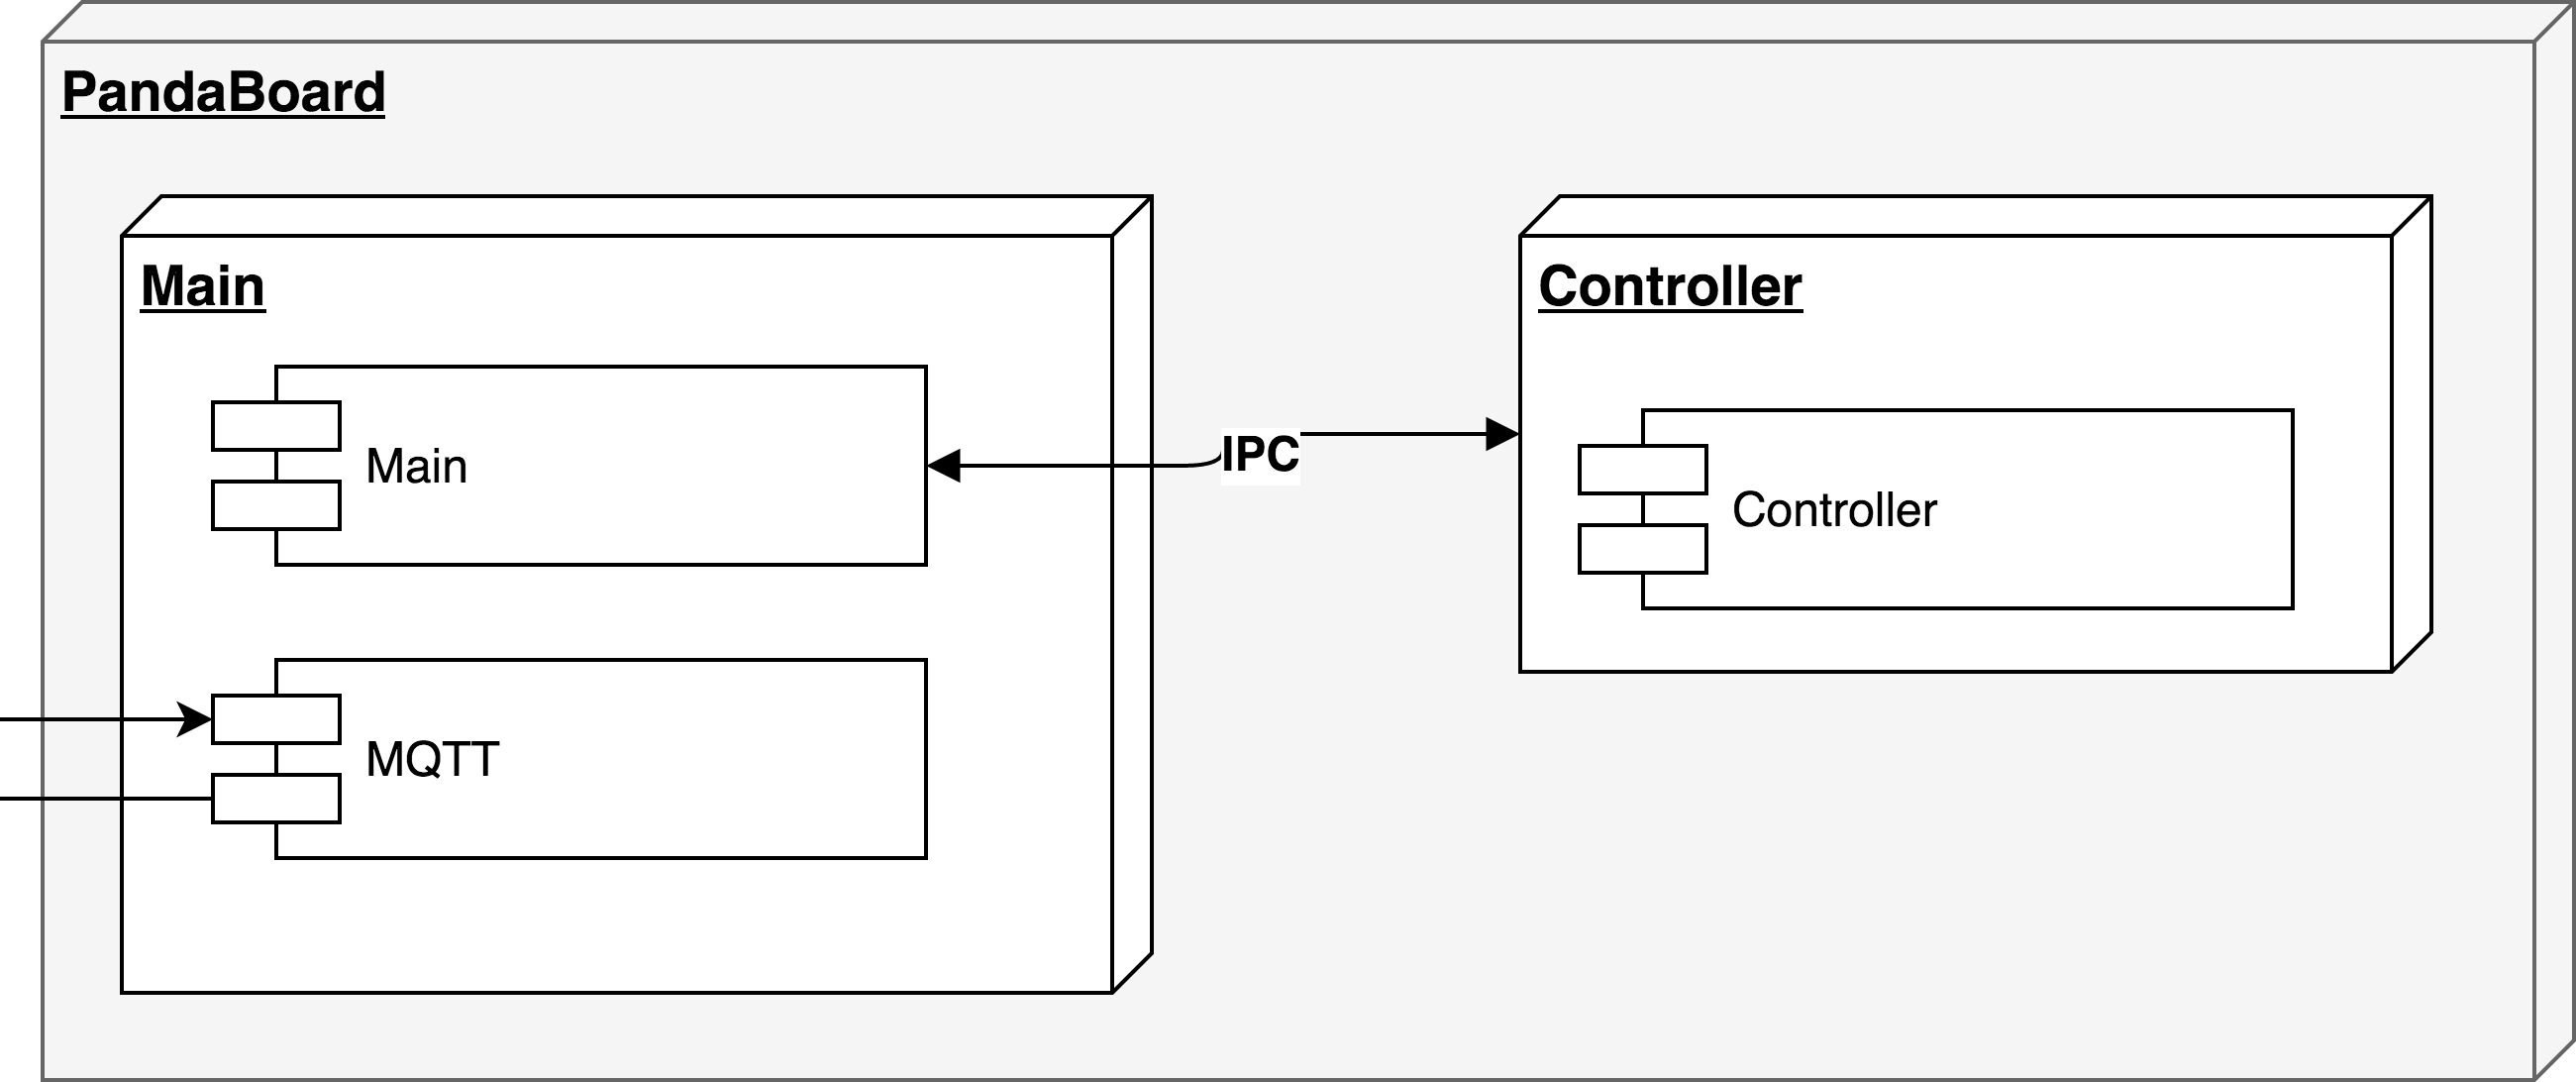
\includegraphics[width=0.7\linewidth]{images/comp_panda}
    \caption{Genode components of the PandaBoard}
    \label{fig:panda-genode}
\end{figure}

The runfile (\texttt{run/car\_panda.run}) contains the build and runtime dependencies as well as configuration settings for individual components.

After startup the \textit{Main} task reads the network configuration from the runfile and configures the network accordingly with either a static IP address or a IP address dynamically obtained over DHCP.

Afterwards it retrieves the IP of the MQTT server from the runfile and attempts to establish a connection.
The task then subscribes to the \textit{car-control} MQTT topic which causes all messages that are published on this topic to be forwarded to the application.

A callback that is executed on reception of every message then copies the data to a buffer where it is in turn processed by the main loop of the task.
After parsing the type of the message, the command is then sent to the responsible function of the \textit{controller task} over IPC.

As all IPC under Genode is synchronous, the \textit{Main} task resumes execution after the function call from the \textit{controller} task returns with the servo adjustment value obtained from the processed command.
The servo value is then published to the \texttt{car-servo} MQTT topic to which the \textit{Raspberry PI} is subscribed and handles all further processing.

% Advantages of genode task

\subsubsection{Command processing}
\label{sec:panda-convert}
The \textit{Control} component is responsible for transforming the messages received in an hardware independent format as described in \autoref{sec:mqtt-car-control} to concrete servo values suited for the servos built into the model car.

\autoref{lst:panda-tsteer} contains the algorithm for calculating the steering servos commands.
First the input value is checked to verify it is within the acceptable input range.
The value is then inverted to ensure correct mapping from the steering direction to the servo direction.
Afterwards the value is transformed by first adjusting the range to $0-1$ and then mapped to the servo input range by multiplying it with the input range of the servo (\textit{SERVO\_UPPER\_BOUND - SERVO\_LOWER\_BOUND}) and then adding the minimum servo value \textit{SERVO\_LOWER\_BOUND}.

As described in \autoref{sec:servo-hard} the minimum servo value is 4000 and the maximum servo value is 8000.
After testing the \textit{SERVO\_LOWER\_BOUND} was set to 4500 while the \textit{SERVO\_UPPER\_BOUND} was set to 7500 to prevent an actuation of the servos beyond the actuation limits of the attached hardware. \\

\begin{minipage}{\linewidth}
\begin{lstlisting}[style=mylistings, language=c, label=lst:panda-tsteer, caption=Algorithm for  calculating the steering servo commands]
int transform_steer(double value) {
	if (value < -1 || value > 1) {
		PERR("Invalid steering angle - range is -1 to 1");
		return -1;
	}

	// Invert value as SpeedDreams thinks -1 is right
	value = -value;

	value = (value + 1)/2;
	return (SERVO_UPPER_BOUND - SERVO_LOWER_BOUND) * value + SERVO_LOWER_BOUND;
}
\end{lstlisting}
\end{minipage} \\

%\begin{minipage}{\linewidth}
%\begin{lstlisting}[style=mylistings, language=c, label=lst:panda-tbreak, caption=Algorithm for calculating the break servo commands]
%int transform_brake(double value) {
%	if (value < 0 || value > 1) {
%		PERR("Invalid target brake position - range is 0 to 1");
%		return -1;
%	}
%
%	return (SERVO_UPPER_BOUND - SERVO_LOWER_BOUND) * value + SERVO_LOWER_BOUND;
%}
%\end{lstlisting}
%\end{minipage} \\


While the current controller only transforms the servo commands and forwards them, the design would also allow more high-level commands from the simulation to be processed where a single control \texttt{car-control} command generates a series of \texttt{car-servo} commands.
One example for this would be ABS style actuation of the servos and relying on sensor data to control the breaking strength.
As no suitable sensor measurements were available during this project, this part has not been implemented.

\subsubsection{Testing}
\label{sec:panda-testing}
To verify the data processing and the actuation of the hardware servos based on control commands sent to the \texttt{car-control} MQTT topic a test script was developed.
This way the hardware side of the HIL setup described in \autoref{sec:intro} can be tested independently of the software side developed by another project team.

The publish–subscribe pattern used by the MQTT server allows multiple clients to simultaneously connect to the server and subscribe to updates on a certain topic or publish messages to a topic.
In this style of communication there are no direct communication links and the components are loosely coupled, simplifying the testing of the interfaces between components.

By using the MQTT commandline tools available under Linux in the \texttt{mosquitto-clients} package message can easily be injected into the \texttt{car-control} topic without changing the configuration of any components.
\autoref{lst:panda-msgpub} shows a small test script that continuously sends steering control messages that cause the steering servos to alternate between actuation to the left and to the right. \\ % when processed by Panda, Rpi and servo components.

\begin{minipage}{\linewidth}
\begin{lstlisting}[style=mylistings, language=c, label=lst:panda-msgpub, caption=Injecting steering commands over MQTT]
#!/usr/bin/env bash
MQTT_IP=$1

while true; do
	mosquitto_pub -h $MQTT_IP -t 'car-control' -m '0,1.0'
	sleep 1
	mosquitto_pub -h $MQTT_IP -t 'car-control' -m '0,-1.0'
	sleep 1
done
\end{lstlisting}
\end{minipage} \\

In a similar manner the \texttt{mosquitto\_sub} commandline tool can be used to subscribe to MQTT topics. This provides easy access to the communication between components for debugging and testing purposes.
\autoref{lst:panda-msgsub} shows the command used to monitor the message published by the panda component. In both listings \texttt{\$MQTT\_IP} is a variable containing the IP address of the MQTT server. \\

\begin{minipage}{\linewidth}
\begin{lstlisting}[style=mylistings, language=c, label=lst:panda-msgsub, caption=Subscribing to MQTT topics]
mosquitto_sub -h $MQTT_IP -t 'car-servo'
\end{lstlisting}
\end{minipage} \\

